\documentclass{article}

\usepackage{graphicx}
\usepackage{tikz}
\usepackage{tikzsymbols}
\usetikzlibrary{calc,patterns,shapes.geometric}
\pagestyle{empty}
\usepackage[margin=0pt]{geometry}
\geometry{papersize={14in,12in}}

\def\centerarc[#1](#2)(#3:#4:#5){\draw[#1] ($(#2)+({#5*cos(#3)},{#5*sin(#3)})$) arc (#3:#4:#5);}

\begin{document}
	\begin{figure}
		\centering
		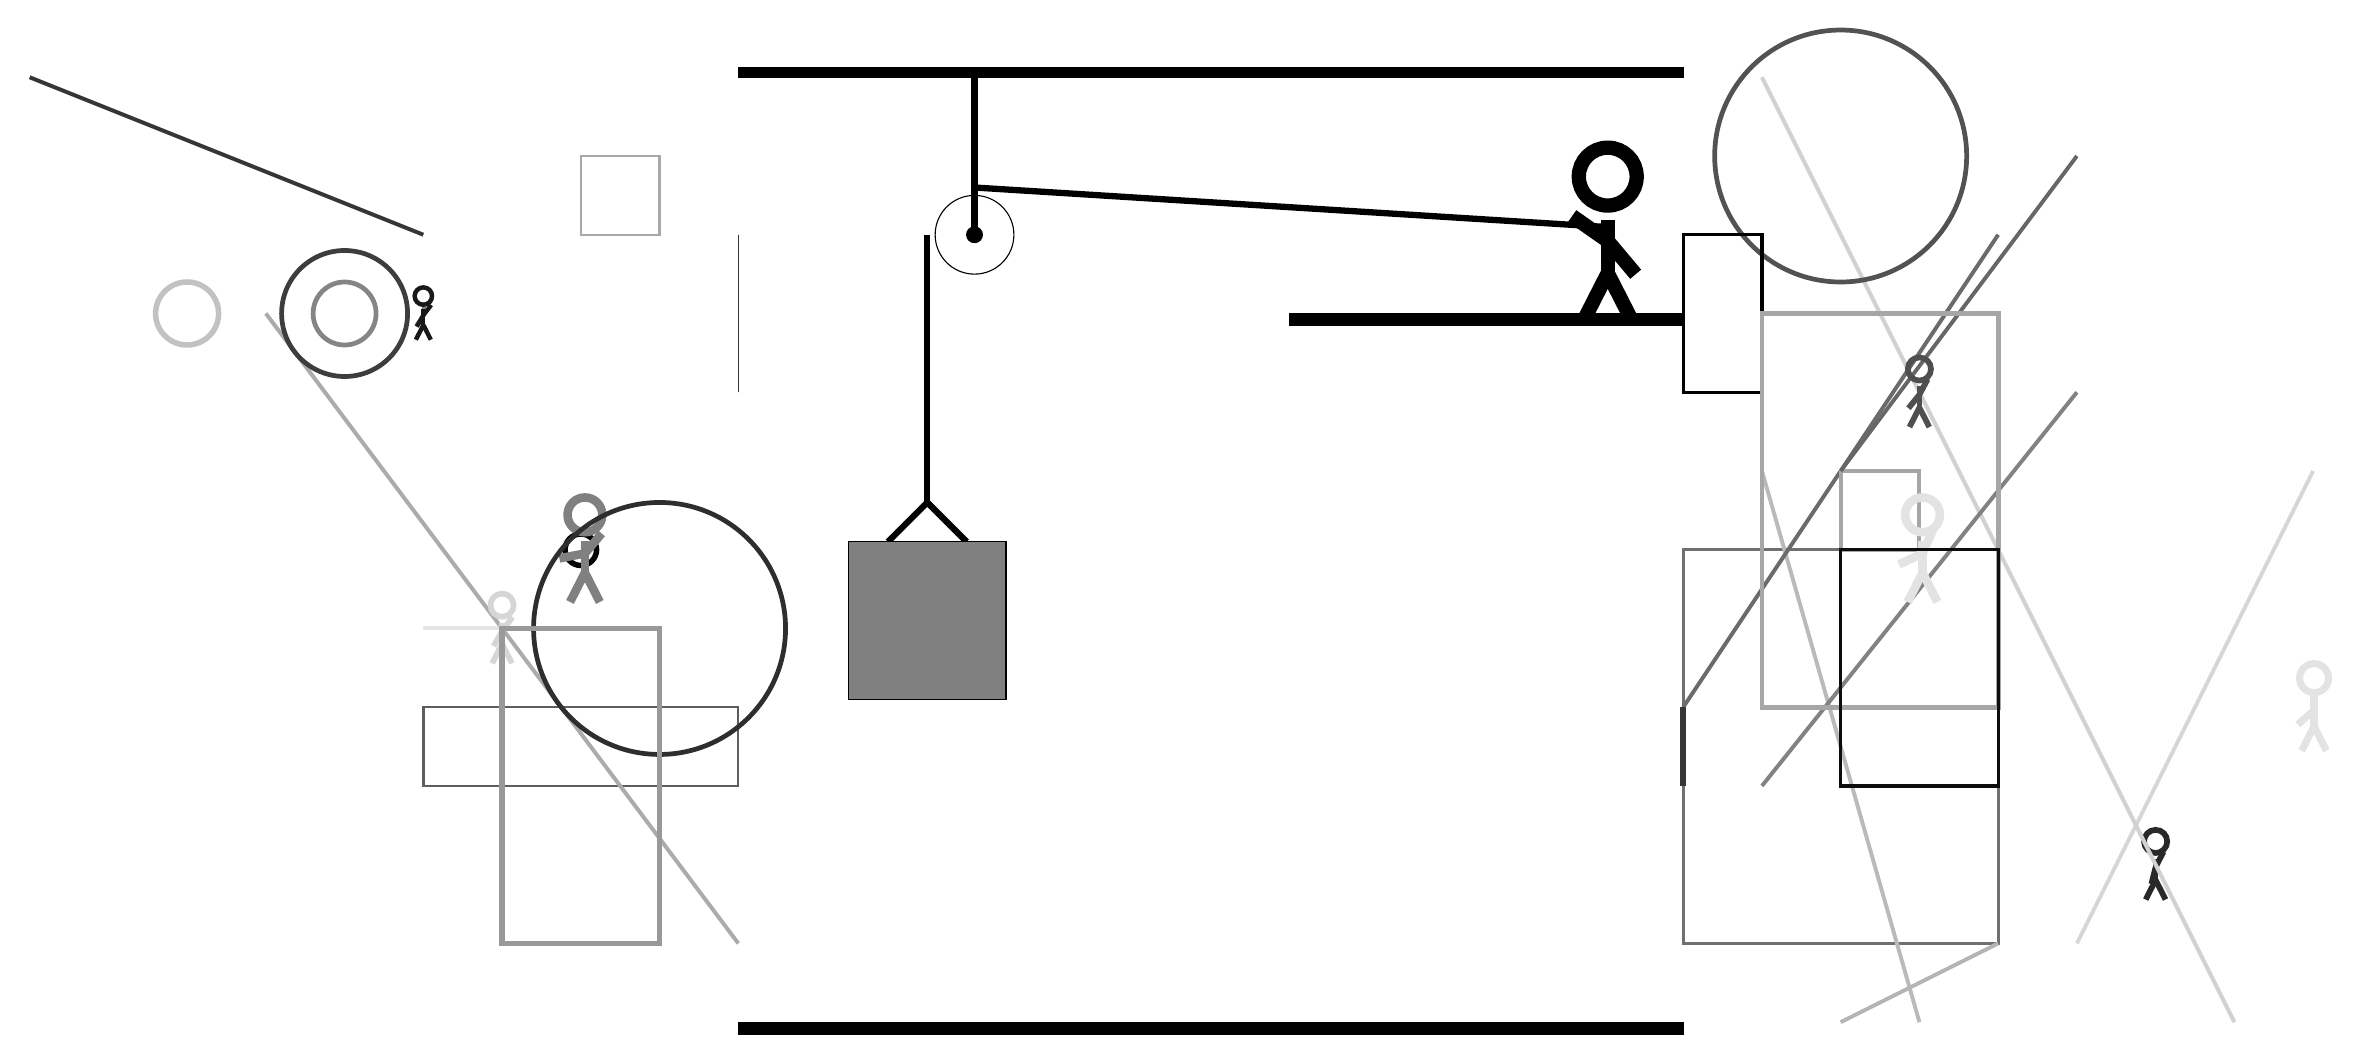
\begin{tikzpicture}
			%%%%% START %%%%%
			
			\draw[fill=black] (-2, 9) rectangle (10, 9.125);
			
			\draw (1, 7) circle (0.5);
			\draw[fill=black] (1, 7) circle (0.1);
			\draw[line width=0.8mm] (1, 9) -- (1, 7);
			
			\draw[line width=0.3mm, color=black!63] (-2, 0) rectangle (-6, 1);
			
			\draw[line width=0.5mm, color=black!16](15, -2) -- (18, 4);
			\draw[line width=0.4mm, color=black!56] (10, 3) rectangle (14, -2);
			\draw[line width=0.5mm, color=black!33](-2, -2) -- (-8, 6);
			\node[line width=0.2mm, color=black!84] at (16, -1) {\Strichmaxerl[4][76][63]};
			
			\draw[line width=0.5mm, color=black!18](11, 9) -- (17, -3);
			
			\draw[line width=0.5mm, color=black!27](13, -3) -- (11, 4);
			
			\node[line width=0.2mm, color=black!11] at (18, 1) {\Strichmaxerl[5][41][90]};
			\draw [line width=0.6mm, color=black!48](-7, 6) circle (0.4);
			
			\draw[line width=0.3mm, color=black!34] (-4, 8) rectangle (-3, 7);
			
			\draw[line width=0.5mm, color=black!29](12, -3) -- (14, -2);
			\draw[line width=0.5mm, color=black!58](14, 7) -- (10, 1);
			\draw[line width=0.2mm, color=black!80] (-2, 5) rectangle (-2, 7);
			
			\draw[line width=0.5mm, color=black!35] (12, 4) rectangle (13, 3);
			\draw [line width=0.6mm, color=black!68](12, 8) circle (1.6);
			\draw[line width=0.5mm, color=black!10](-5, 2) -- (-6, 2);
			
			\draw[line width=0.5mm, color=black!49](11, 0) -- (15, 5);
			\draw [line width=0.7mm, color=black!98](-4, 3) circle (0.2);
			\node[line width=0.2mm, color=black!16] at (-5, 2) {\Strichmaxerl[4][61][53]};
			\node[line width=0.7mm, color=black!50] at (-4, 3) {\Strichmaxerl[6][11][50]};
			\draw [line width=0.7mm, color=black!24](-9, 6) circle (0.4);
			\draw[line width=0.5mm, color=black!60](12, 4) -- (15, 8);
			\draw [line width=0.6mm, color=black!82](-3, 2) circle (1.6);
			\node[line width=0.5mm, color=black!69] at (13, 5) {\Strichmaxerl[4][51][62]};
			\draw[line width=0.4mm, color=black!100] (10, 5) rectangle (11, 7);
			\node[line width=0.3mm, color=black!48] at (-6, 6) {\Strichmaxerl[3][56][85]};
			\draw[line width=0.6mm, color=black!35] (11, 1) rectangle (14, 6);
			\draw[line width=0.7mm, color=black!40] (-3, -2) rectangle (-5, 2);
			
			\draw [line width=0.6mm, color=black!76](-7, 6) circle (0.8);
			\node[line width=0.2mm, color=black!11] at (13, 3) {\Strichmaxerl[6][25][66]};
			\draw[line width=0.4mm, color=black!95] (12, 3) rectangle (14, 0);
			
			\draw [line width=0.2mm, color=black!30](-8, -2) circle (0.0);
			\node[line width=0.3mm, color=black!90] at (-6, 6) {\Strichmaxerl[3][60][53]};
			\draw[line width=0.5mm, color=black!79](-6, 7) -- (-11, 9);
			
			\draw[line width=0.7mm, color=black!79] (10, 0) rectangle (10, 1);
			
			\draw[line width=0.8mm](-0.1, 3.1) --  (0.4, 3.6) -- (0.9, 3.1);
			\draw[fill=black!50] (-0.6, 3.1) rectangle (1.4, 1.1);
			
			\draw[line width=0.8mm](0.4, 7) -- (0.4, 3.6);
			\centerarc[line width=0.8mm](1, 7)(90:180:0.6)
			\draw[line width=0.8mm](1, 7.6) -- (9, 7.1);
			
			\node at (9, 7) {\Strichmaxerl[10][-35][-50]};
			\draw[fill=black] (5, 6) rectangle (10, 5.85);
			
			\draw[fill=black] (-2, -3) rectangle (10, -3.15);
			
			%%%%% END %%%%%
		\end{tikzpicture}
	\end{figure}	
\end{document}